\begin{multicols*}{2}
\section*{9. Natural Convection}
\subsection*{9.1. General Procedure}
\subsubsection*{9.1.1. Over Surfaces}
\begin{enumerate}
    \item Find Rayleigh number, Ra$_L$, using fluid properties at film temperature $T_f = (T_s + T_\infty)/2$
    \item Use the appropriate correlation in Table \ref{tab:sec9_natural_convection_over_surfaces} 
    to find the Nusselt number, Nu
    \item Determine the heat transfer coefficient $h$ using Nu, $k$, and $L_c$
\end{enumerate}
\subsubsection*{9.1.2. In Enclosures}
\begin{enumerate}
    \item Find Rayleigh number, Ra$_L$, using fluid properties at average temperature $T_{\text{avg}} = (T_1 + T_2)/2$
    where $T_1$ and $T_2$ are the temperatures of the hot and cold surfaces respectively.
    \item Use the appropriate correlation to find the Nusselt number, Nu
    \item Determine the heat transfer coefficient $h$ using Nu, $k$, and $L_c$
\end{enumerate}
% Add this to a glossary section later
\subsection*{9.2. Variable Definitions}
\begin{itemize}
    % \item Nu: Nusselt number
    % \item Re: Reynolds number
    % \item Pr: Prandtl number
    % \item $\mu$: Dynamic viscosity
    % \item $\nu$: Kinematic viscosity
    % \item $k$: Thermal conductivity
    % \item $h$: Convection heat transfer coefficient
    % \item $D_h$: Hydraulic diameter
    % \item $A_s$: Surface area
    % \item $A_c$: Cross-sectional area
    % \item $V_{\text{avg}}$: Average velocity
    % \item $T_b$: Bulk mean temperature
    % \item $T_i$: Inlet temperature
    % \item $T_e$: Exit temperature
    % \item $\dot{m}$: Mass flow rate
    % \item $\dot{q}$: Heat flux 
    % \item $\Delta T_{\text{lm}}$: Log mean temperature difference   
    \item Ra$_L$: Rayleigh number
    \item Gr$_L$: Grashof number
    \item $T_s$: Surface temperature
    \item $T_\infty$: Ambient temperature
    \item $T_f$: Film temperature
    \item $L_c$: Characteristic length
    \item $\beta$: Coefficient of volume expansion
    \item $\nu$: Kinematic viscosity
    \item $\alpha$: Thermal diffusivity
    \item $g$: Gravitational acceleration
\end{itemize}

\subsection*{9.3. Formulas}
\begin{align*}
    \text{Ra}_L &= \text{Gr}_L \text{Pr} = \frac{g \beta (T_s - T_\infty) L_c^3}{\nu^2} \text{Pr} \\
    \beta &= \frac{1}{T}, \quad \text{for ideal gases} \\
    h &= \frac{k \text{Nu}}{L_c} 
\end{align*}
\subsubsection*{9.3.1. Over Surfaces}
For convection 
\begin{align*}
    \dot{Q} &= h A_s (T_s - T_\infty)
\end{align*}
Use Table \ref{tab:sec9_natural_convection_over_surfaces} to find Nu.
\subsubsection*{9.3.2. In Rectangular Enclosures}
For convection in rectilinear enclosures, 
\begin{equation*}
    \dot{Q} = h A_s (T_1 - T_2) 
\end{equation*}
where $T_1$ and $T_2$ are the temperatures of the hot and cold surfaces respectively.

In \textbf{horizontal rectangular enclosures} ($L_c = L$, where $L$ is the gap between plates),
\begin{gather*}
    \text{Nu} = 1 + 1.44 \left[1 - \left(\frac{1708}{\text{Ra}_L}\right)\right]^{+} + \left[\frac{\text{Ra}_L}{18} - 1\right]^{+}\\
    \text{Ra}_L < 10^8 \; (\text{gases}), \quad \text{Ra}_L < 10^{5} \; (\text{liquids})
\end{gather*}
For large aspect ratios ($H/L \geq 12$), this equation (Hollands et al., 1976) correlates experimental data extremely well for tilt angles up to 70$^{\circ}$.
$\left[ \;\right]^+$ indicates that if the quantity in the bracket is negative, it should be set equal to zero.
\begin{gather*}
    \text{Nu}_L = 1 + 1.44 \left[1 - \left(\frac{1708}{\text{Ra}_L \cos\theta}\right)\right]^{+} + \left[\frac{\text{Ra}_L \cos\theta}{18} - 1\right]^{+}\\
    \text{Ra}_L < 10^8 \; (\text{gases}), \quad \text{Ra}_L < 10^{5} \; (\text{liquids}), \\
    0 < \theta < 70^{\circ}, \quad \frac{H}{L} \geq 12
\end{gather*}
In \textbf{vertical rectangular enclosures} ($L_c = L$, where $L$ is the gap between plates),
\begin{gather*}
    \text{Nu}_L = 0.18\left(\frac{\text{Pr}}{0.2 + \text{Pr}} \text{Ra}_L \right)^{0.29}\\
    \frac{\text{Pr}}{0.2 + \text{Pr}} > 10^3, \; 1 < \frac{H}{L} < 2 
\end{gather*}
or 
\begin{gather*}
    \text{Nu}_L = 0.22\left(\frac{\text{Pr}}{0.2 + \text{Pr}} \text{Ra}_L \right)^{0.28} \left(\frac{H}{L}\right)^{-0.25}\\
    \text{Ra}_L < 10^{10}, \; 2 < \frac{H}{L} < 10
\end{gather*}
or
\begin{gather*}
    \text{Nu}_L = 0.42\left(\frac{\text{Pr}}{0.2 + \text{Pr}} \text{Ra}_L \right)^{0.25}\text{Pr}^{0.012} \left(\frac{H}{L}\right)^{-0.3}\\
    1 < \text{Pr} < 2 \times 10^4, \; 10^4 < \text{Ra}_L < 10^7, \; 10 < \frac{H}{L} < 40
\end{gather*}
\subsubsection*{9.3.3. In Concentric Horizontal Cylinders}
In \textbf{concentric horizontal cylinders} ($L_c = (D_o - D_i)/2$, where $D_o$ and $D_i$ are the outer and inner diameters respectively),
\begin{equation*}
    \dot{Q}_{\text{cylinder}} = \frac{2\pi k \text{Nu}}{\ln(D_o/D_i)}(T_i - T_o) 
\end{equation*}
where $T_i$ and $T_o$ are the temperatures of the inner and outer surfaces respectively.
\begin{gather*}
    \text{Nu} = \max\left\{1, \;0.386 \left(\frac{\text{Pr}}{0.861 + \text{Pr}}\right)^{0.25}(F_{\text{cyl}} \text{Ra}_L)^{0.25}\right\}\\
    %\text{Nu} = \max\left{1, \right}
    %0.386 \left(\frac{\text{Pr}}{0.861 + \text{Pr}}\right)^{0.25}(F_{\text{cyl}} \text{Ra}_L)^{0.25}
%     F_{\text{cyl}} = \frac{\ln^4(D_o/D_i)}{L_{c}^3 (D_{i}^{-0.6}+D_{o}^{-0.6})^5} 
\end{gather*}
\subsubsection*{9.3.4. Combined Natural and Forced Convection}
For combined natural and forced convection, 
\begin{equation*}
    \text{Nu}_{\text{Overall}} = \left(\text{Nu}_{\text{Forced}}^n \pm \text{Nu}_{\text{Natural}}^n\right)^{1/n}
\end{equation*}
where the plus sign is for assisting flows and the minus sign is for opposing flows. $n = 3.5$ for 
horizontal plates and $n = 4$ for cylinders and spheres. Else use $n = 3$.
\end{multicols*}

\section*{Tables}
% \begin{table}[H]
%     \centering
%     \caption{Empirical correlations for the average Nusselt number for natural convection over surfaces 
%     (\textbf{Table 9-1 in textbook})}
%     \label{tab:sec9_natural_convection_over_surfaces}
%     \begin{tabular}{p{0.2\textwidth}p{0.1\textwidth}p{0.15\textwidth}p{0.4\textwidth}}
%         \hline
%         Geometry & Characteristic Length $L_c$ & Range & Nu \\
%         \hline
%         \multirow{2}{*}{Vertical Plate 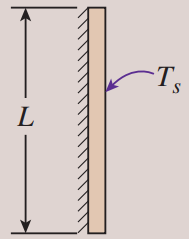
\includegraphics[width=0.1\textwidth]{Figures/Sec9 Vertical Plate.png}} 
%         & $L$ & $10^4 \leq \text{Ra}_L \leq 10^{9}$ & $\displaystyle \text{Nu} =0.59 \text{Ra}_L^{1/4}$ \\
%         & & $\displaystyle 10^{9} \leq \text{Ra}_L \leq 10^{13}$ & $\text{Nu} = 0.1 \text{Ra}_L^{1/3}$ \\
%         & & Entire range & $\displaystyle \text{Nu} = \left(0.825 + \frac{0.387 \text{Ra}_L^{1/6}}{[1 + (0.492/\text{Pr})^{9/16}]^{8/27}}\right)^2$ \\
%         & & & (complex but more accurate) \\
%         & & & \\
%         \hline
%         \multirow{2}{*}{Inclined Plate 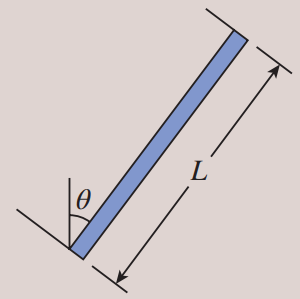
\includegraphics[width=0.1\textwidth]{Figures/Sec9 Inclined Plate.png}}
%         & $L$ & & Use vertical plate equations for the upper 
%         surface of a cold plate and the lower 
%         surface of a hot plate \\
%         & & & \\
%         & & & Replace $g$ with $g \cos\theta$ for $0 < \theta < 60^\circ$ \\
%         & & & \\
%         \hline
%         % finish later
%     \end{tabular}
% \end{table}
\begin{table}[H]
    \centering
    \caption{Empirical correlations for the average Nusselt number for natural convection over surfaces 
    (\textbf{Table 9-1 in textbook})}
    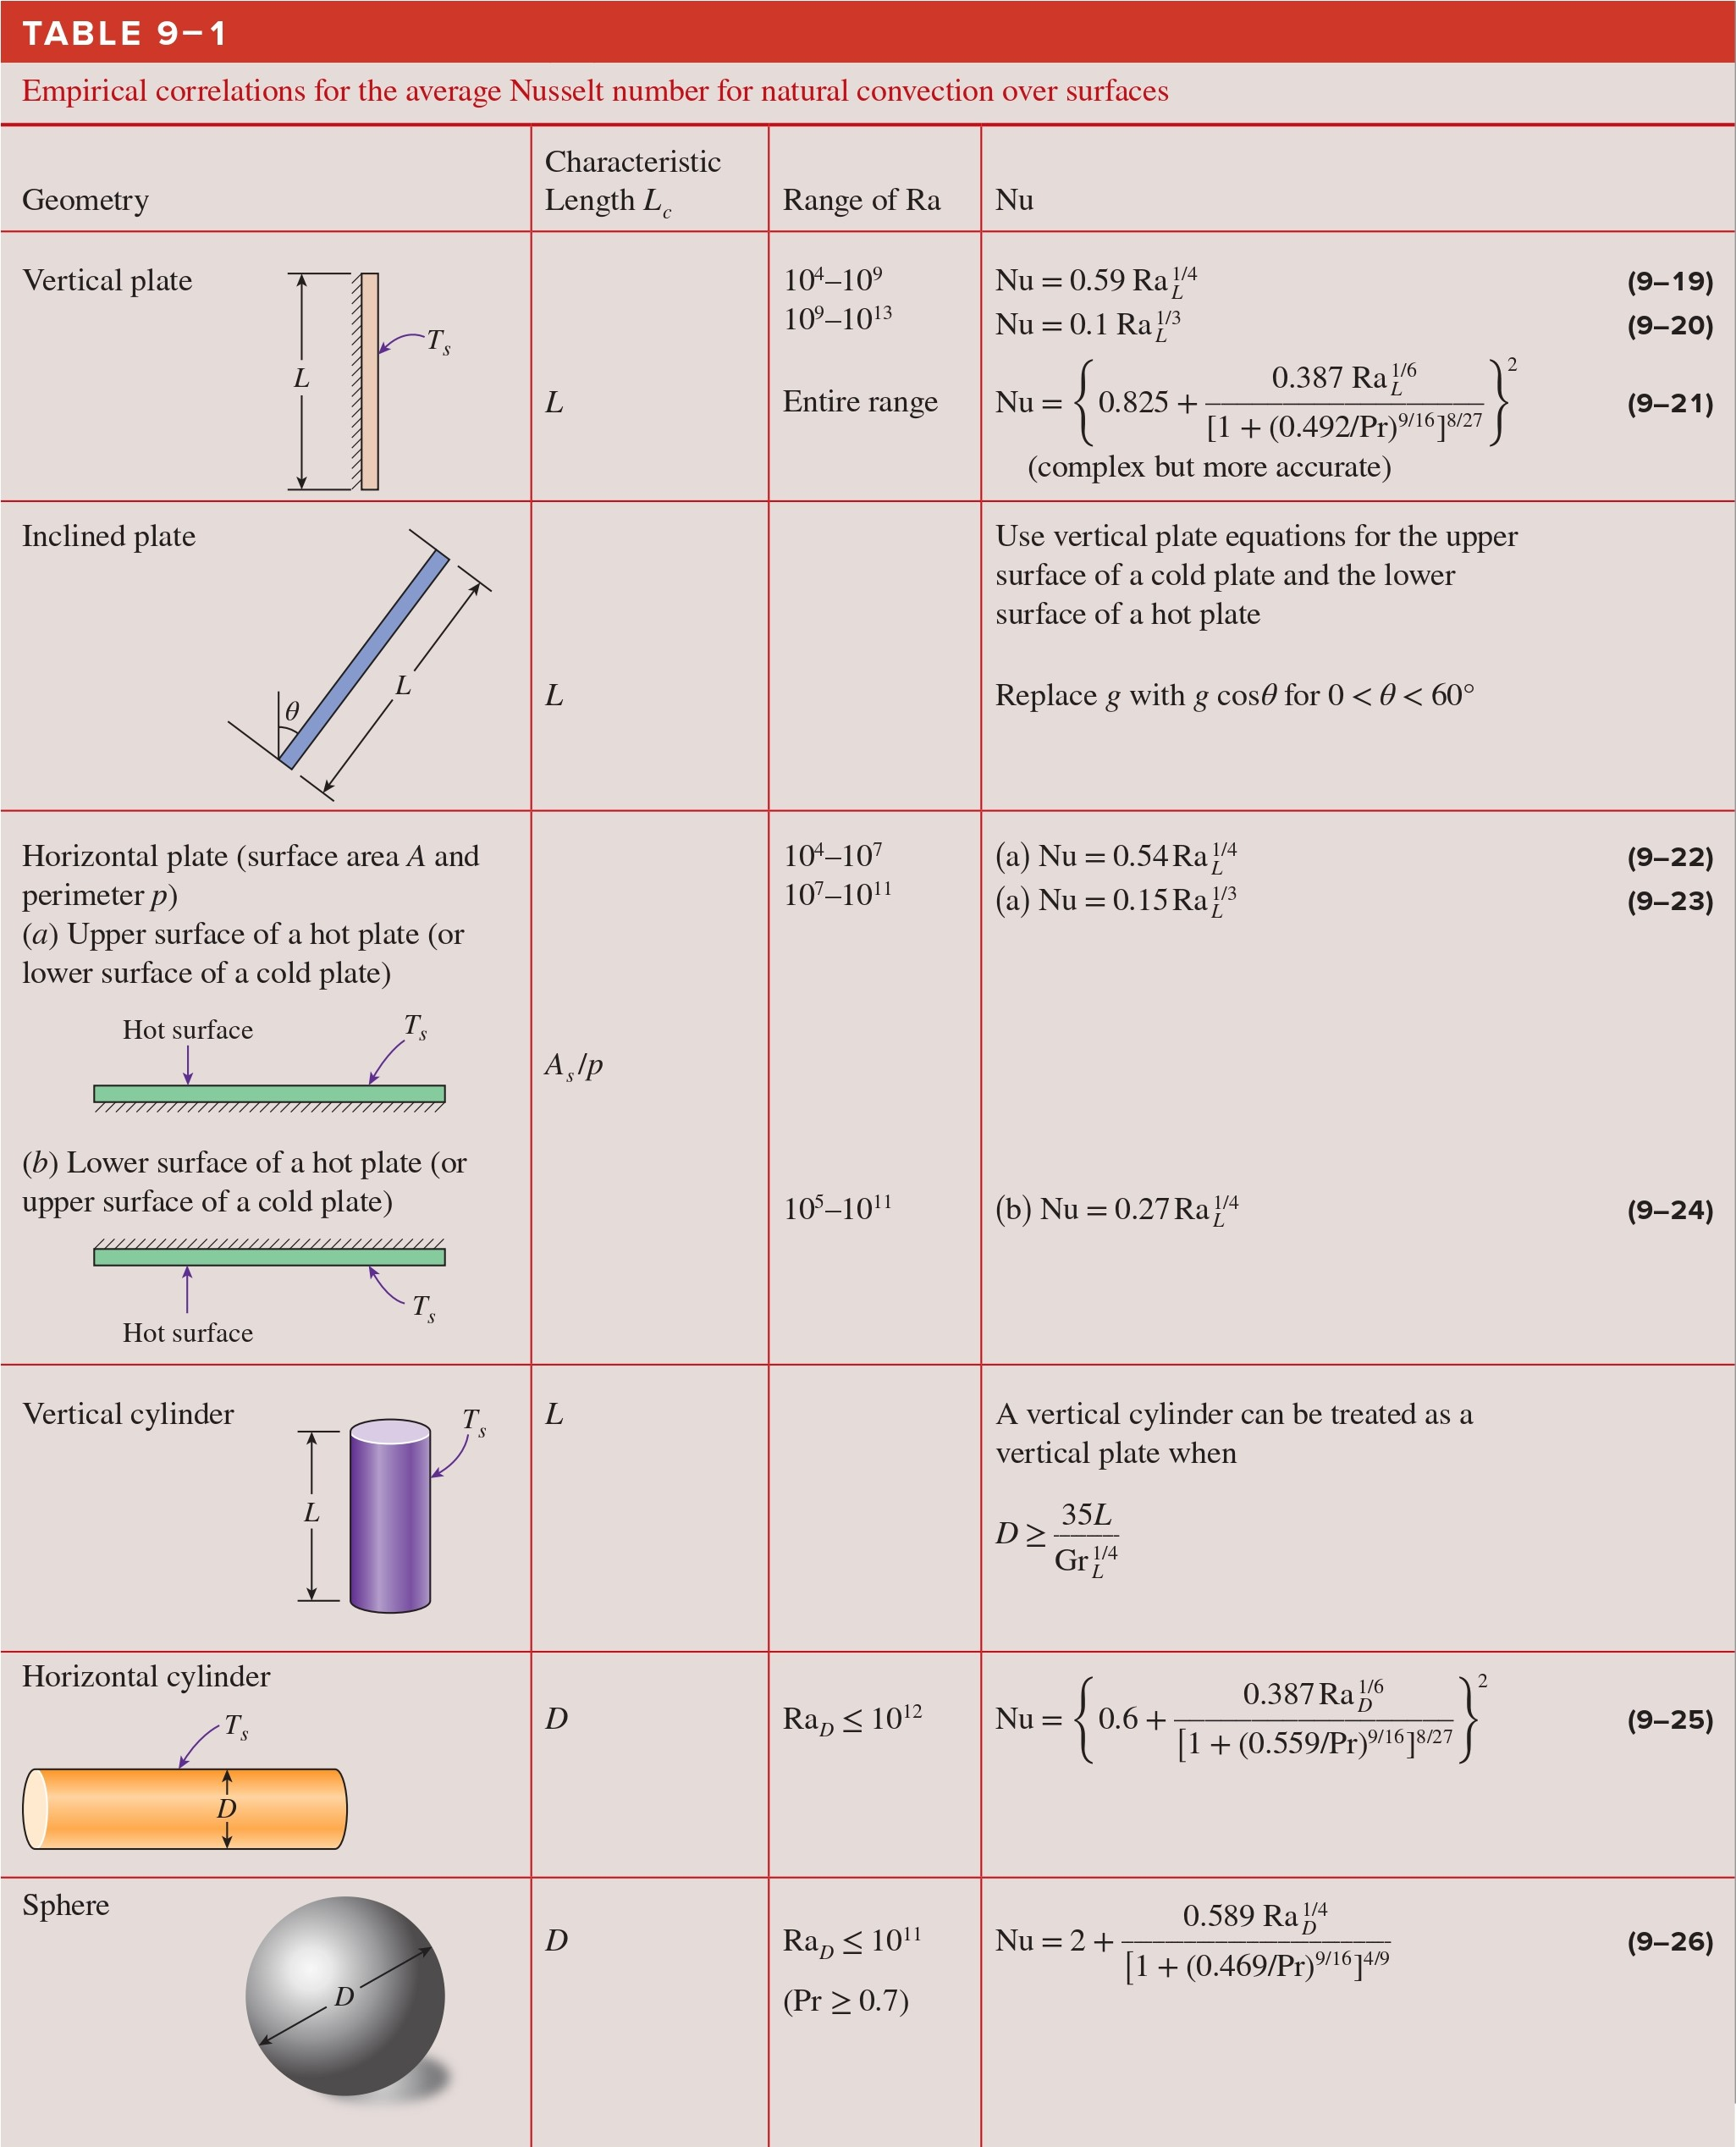
\includegraphics[width=0.8\textwidth]{Figures/sec9 table 9-1.jpg}
    \label{tab:sec9_natural_convection_over_surfaces}
\end{table}

% %     \centering
%     \caption{Nusselt number and friction factor for fully developed laminar flow in tubes of various cross sections 
%     ($D_h = 4A_c /P$, $Re = V_{\text{avg}} D_h / \nu$, and $\text{Nu} = hD_h / k$) (\textbf{Table 8-1 in textbook})}
%     \label{tab:sec8_fully_developed_laminar}
%     \begin{tabular}{ccccc}
%         \hline
%         & & \multicolumn{2}{c}{Nu} & \\
%         \cline{3-4}
%         Tube Geometry & $a/b$ or $\theta^\circ$ & $T_s = \text{constant}$ & $\dot{q}_s = \text{constant}$ & $f$ \\
%         \hline
%         \raisebox{-\totalheight}{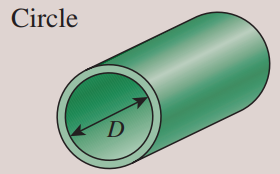
\includegraphics[width=0.15\textwidth]{Figures/Sec8 Circle Fully Laminar.png}} & --- & 4.36 & 3.66 & 64/Re \\
%         \hline
%         & \underline{$a/b$} & & & \\ 
%         \multirow{2}{*}{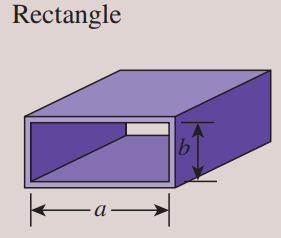
\includegraphics[width=0.15\textwidth]{Figures/Sec8 Rectangle Fully Laminar.png}} 
%         & 1 & 2.98 & 3.61 & 56.92/Re \\
%         & 2 & 3.39 & 4.12 & 62.20/Re \\
%         & 3 & 3.96 & 4.79 & 68.36/Re \\
%         & 4 & 4.44 & 5.33 & 72.92/Re \\
%         & 6 & 5.14 & 6.05 & 78.80/Re \\
%         & 8 & 5.60 & 6.49 & 82.32/Re \\
%         & $\infty$ & 7.54 & 8.24 & 96.00/Re \\
%         \hline
%         & \underline{$a/b$} & & & \\
%         \multirow{2}{*}{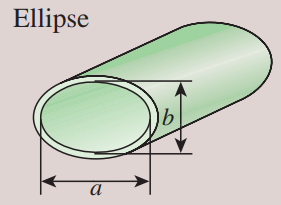
\includegraphics[width=0.15\textwidth]{Figures/Sec8 Ellipse Fully Laminar.png}}
%         & 1 & 3.66 & 4.36 & 64.00/Re \\
%         & 2 & 3.74 & 4.56 & 67.28/Re \\
%         & 4 & 3.79 & 4.88 & 72.96/Re \\
%         & 8 & 3.72 & 5.09 & 76.60/Re \\
%         & 16 & 3.65 & 5.18 & 78.16/Re \\
%         \hline
%         & \underline{$\theta^\circ$} & & & \\
%         \multirow{2}{*}{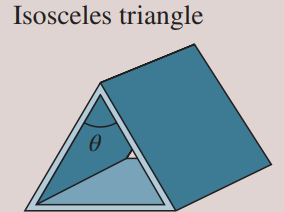
\includegraphics[width=0.15\textwidth]{Figures/Sec8 Triangle Fully Laminar.png}}
%         & 10 & 1.61 & 2.45 & 50.80/Re \\
%         & 30 & 2.26 & 2.91 & 52.28/Re \\
%         & 60 & 2.47 & 3.11 & 53.32/Re \\
%         & 90 & 2.34 & 2.98 & 52.60/Re \\
%         & 120 & 2.00 & 2.68 & 50.96/Re \\
%         \hline
%         % \raisebox{-\totalheight}{\includegraphics[width=0.15\textwidth]{Figures/Sec8 Square Fully Laminar.png}} & 1 & 3.66 & 3.11 & 64/Re \\
%     \end{tabular}